% [11~v\textsuperscript{o}]
\pstart%
In pullo ex ovo sponte
\edtext{egresso, sed}{\lemma{egresso,}\Bfootnote{\textit{(1)}\ et \textit{(2)}\ sed \textit{L}}}
qui nondum comederat, notavi pulmones
\edtext{[costis]}{\lemma{rostris}\Bfootnote{\textit{L \"{a}ndert Hrsg.}}}
utrinque firmiter adhaerere et infra dia$\phi$ragma etiam aliquid utrinque costis firmiter adhaerere quod putavi pro liene esse sumendum;
hujusque sinistra pars paulo magis ex rubro nigrescens videbatur; quam dextra pulmones adhuc magis rubebant et nigrescebant itemque cordis auriculae ambae. Paulo minus rubebat hepar aequaliter in utrumque latus positum, hujusque pars dextra, cui vesicula fellis innascebatur, aliquo modo flavescebat. Cor erat multo magis album, hujus dextra cavitas multo magis curvata, quam in pullo, sed cujus paries exterior vix tenuior videbatur quam parietes sinistrae cavitatis, qui tamen in adultis sunt decuplo crassiores. Infra hepar apparebat ventriculus plane albus, in quo aliquid materiae ex flavo virescens, conspiciebatur
\edtext{postquam erat}{\lemma{postquam}\Bfootnote{\textit{(1)}\ esset \textit{(2)}\ erat \textit{L}}}
apertus ei appendebant intestina umbilicus, et a podice erat satis
\edtext{remotus et}{\lemma{remotus}\Bfootnote{\textit{(1)}\ ex \textit{(2)}\ et \textit{L}}}
juxta illum in ventris capacitate continebatur ovi vitellus vix tertia parte imminutus, eoque cocto inveni esse ejusdem saporis, sed multo durioris substantiae quam ovorum recentium. Pendebat autem ille vitellus ex vase quodam inter intestina misto, et nondum notare potui an in hepate vel alibi terminaretur. Albumen etiam nullum vidi sed totum erat consumtum.
\pend%
\pstart%
Ita judico per albumen spiritus animales spargi atque in eo tanquam in semine quadrupedum membra prius formari saltem in ejus chalaza initio ac deinde paulatim in reliquo, adeo ut ejus ultimis
\edtext{partibus omnium}{\lemma{}\Afootnote{\textit{Zwischen} partibus omnium: \Denarius \vspace{-4mm}}}
ultima cutis circa umbilicum formetur.
\pend%
\pstart%
Venae et arteriae non fiunt nisi juxta tunicas vitelli et albuminis quae videntur esse instar duarum tunicarum foetum quadrupedum involventium.
\pend%
\newpage
\pstart%
Cor non formatur in medio seminis, sed potius in aliqua extremitate ut
\edtext{videmus in plantarum seminibus}{\lemma{videmus in}\Bfootnote{\textit{(1)}\ medio \textit{(2)}\ plantarum seminibus \textit{L}}}
partem quae germinat semper esse in extremitate aliqua.
\pend%
\pstart%
Cursus sanguinis in vena coronaria et dextro ventriculo volvitur in orbem ut cochleae omnes, itemque ut gerania et faseoli, sed contrario modo quam convolvulus.
\pend%
\pstart%
In pisce cabeliau fauces erant multo ampliores quam gula, gula quam ventriculus; intestina etiam
\rule[-2mm]{0mm}{13mm}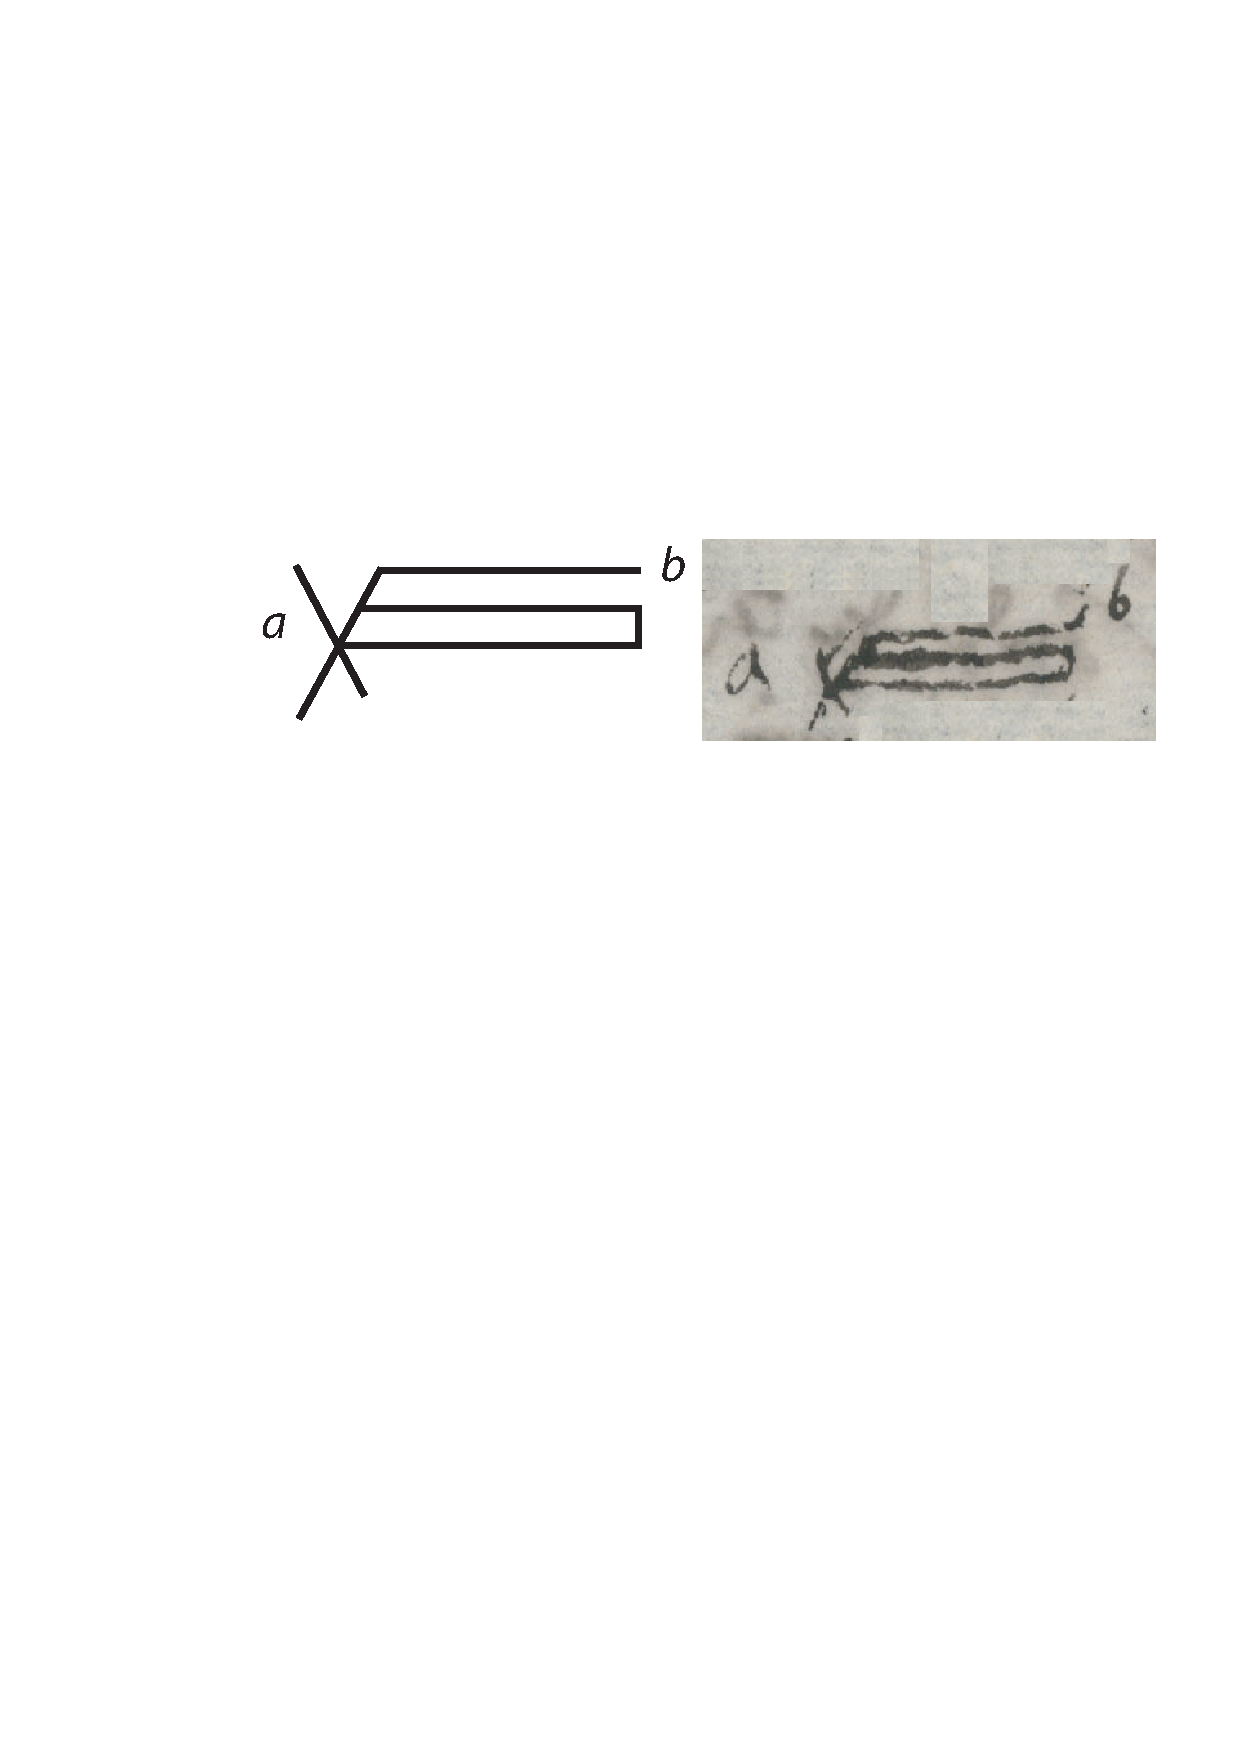
\includegraphics[width=0.3\textwidth]{images/lh0040104b_011v1.pdf}
erant satis angusta, et in tres tantum plicas intorta; ut in hac figura, $a$ ventriculus; $b$ podex. Constabat autem ventriculus fibris permultis, tanquam in palato bovis extantibus et multo longioribus. Fel adhaerebat partim istis fibris partim intestino, lien erat infra fel et intestino etiam adhaerebat; hepar erat valde album, et non notavi an alibi quam cordi adhaereret; haerebat autem cordi ope venae cavae valde brevis quae versus cor admodum protuberabat ita ut iste tumor auriculae vicem subiret, a corde egrediebatur aorta etiam valde protuberans
\rule[-2mm]{0mm}{11mm}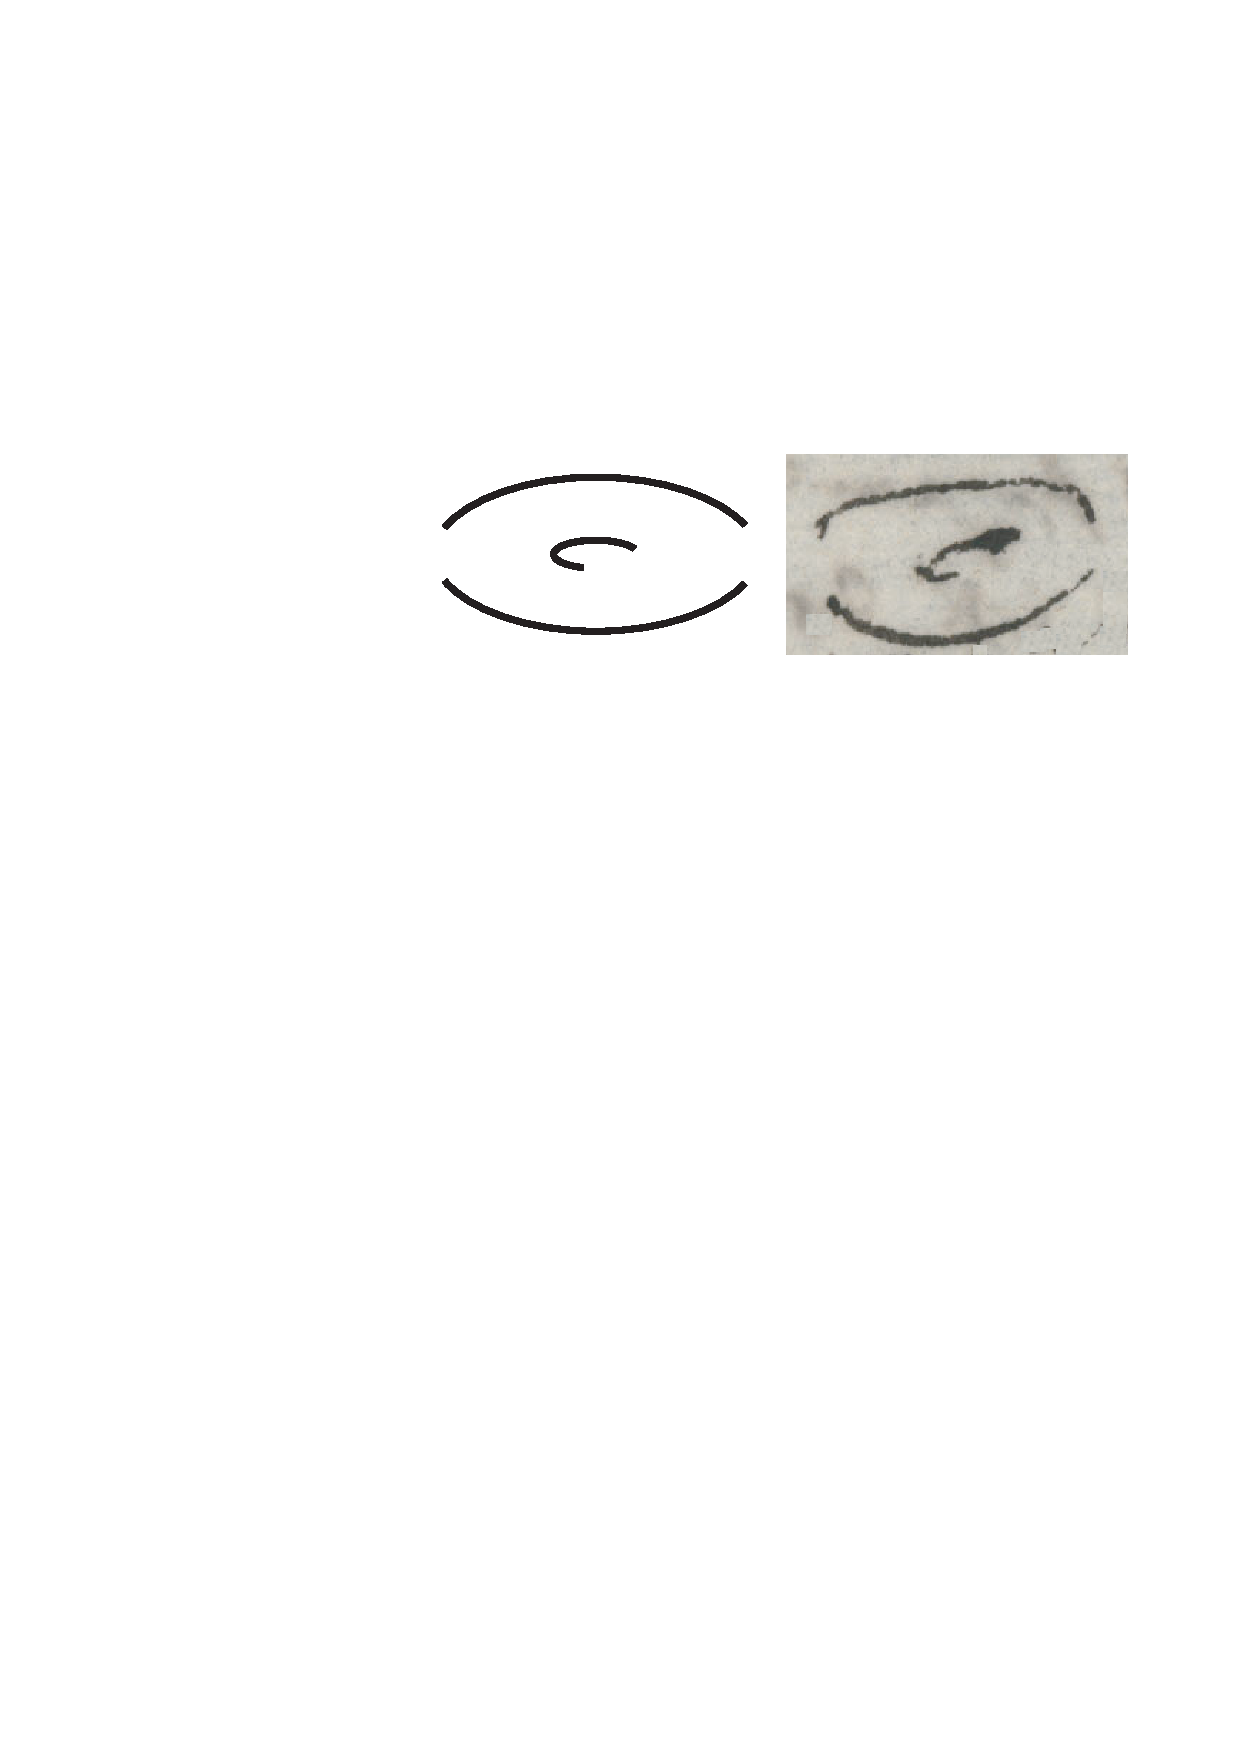
\includegraphics[width=0.2\textwidth]{images/lh0040104b_011v2.pdf}
non longior neque crassior quam hic pingitur
\rule[-2mm]{0mm}{10mm}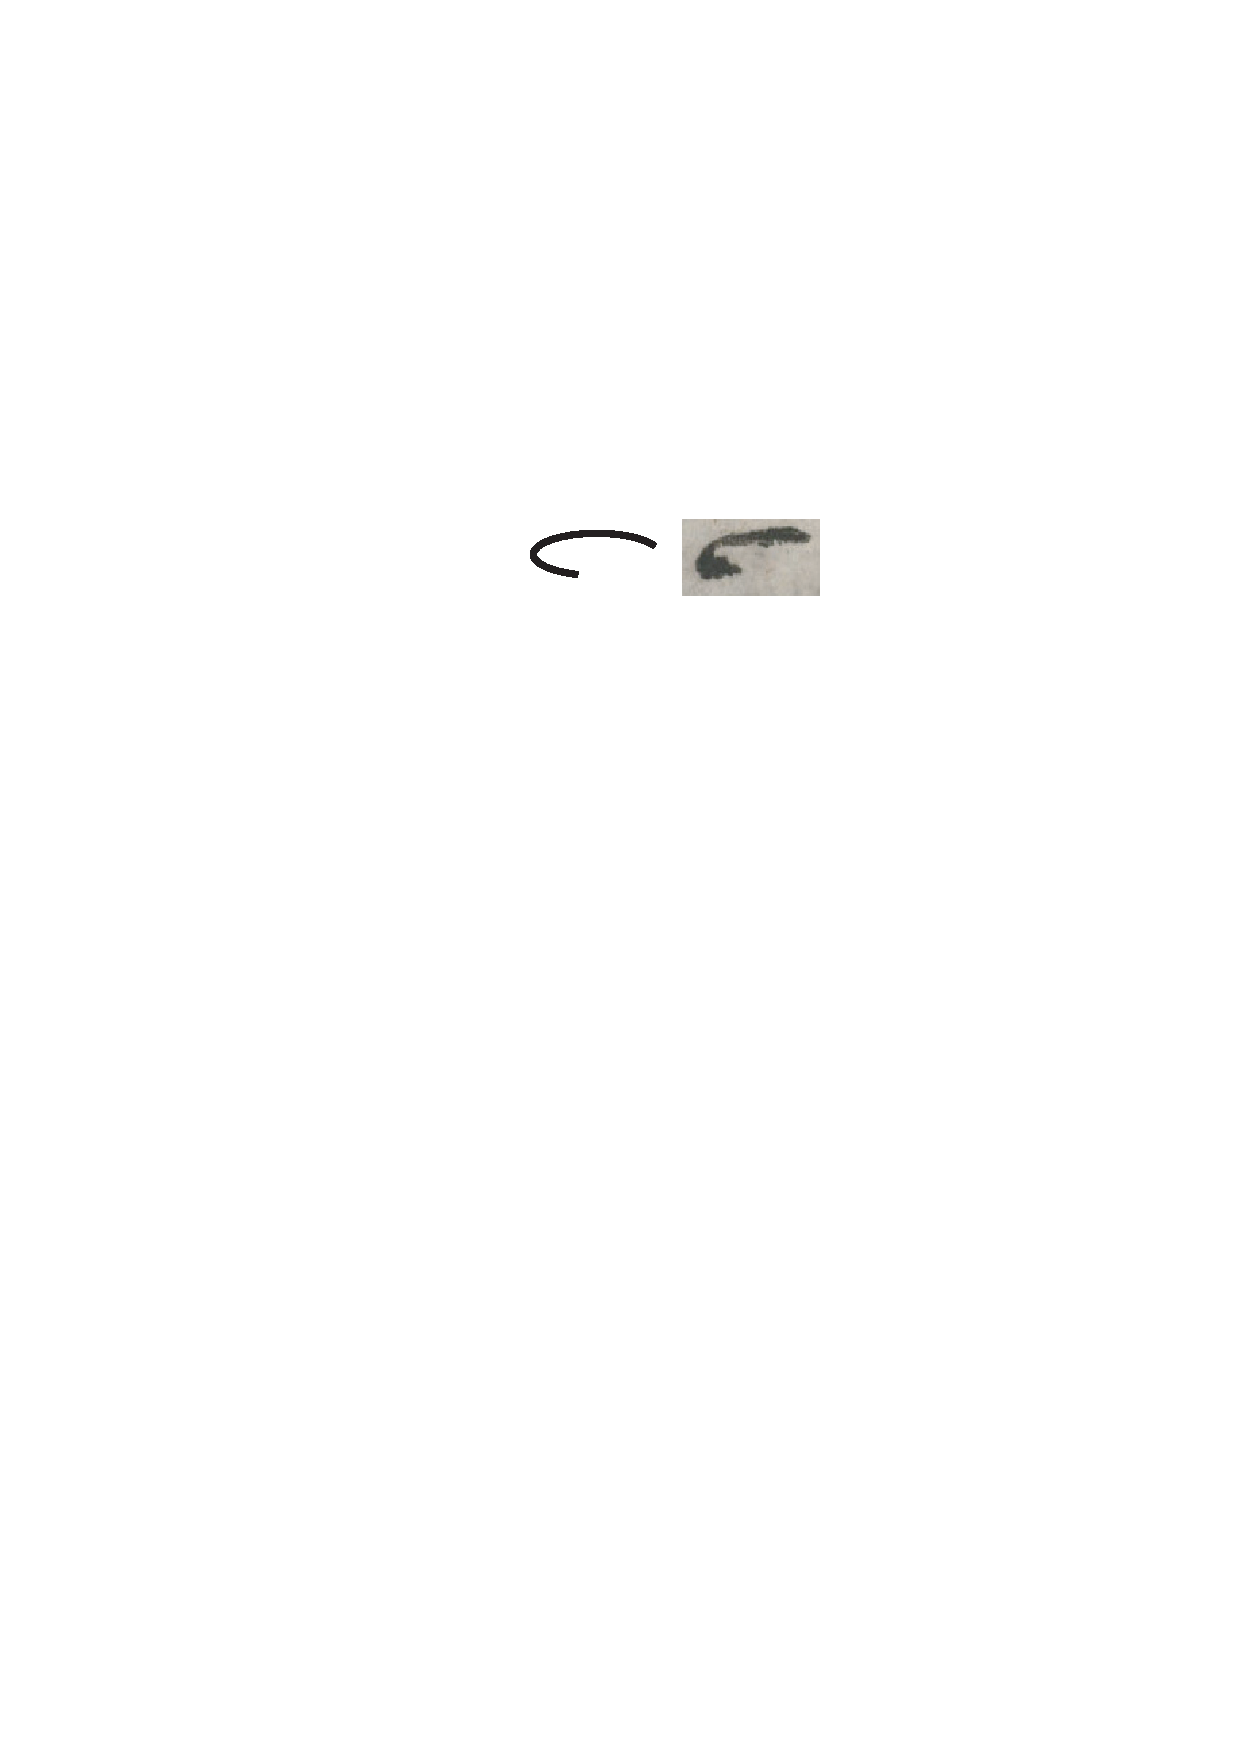
\includegraphics[width=0.2\textwidth]{images/lh0040104b_011v3.pdf}
piscis autem erat circiter trium palmarum longitudinis, et affixa erat anteriori et infimae oris parti, ubi in carnes dispergebatur, adeo ut facile crediderim sanguinem in istis animalibus non circulari; fel erat caeruleum, lien valde rubens et vividum, hepar vero album, quo confirmor in ea opinione, quod ex liene sanguis veniens ad hepar chylo misceatur, qui chylus non fit ruber nisi in corde. Nec multo hepate isti pisces opus habent.
\pend%
\pstart%
In pisce Schelfisch ex maximis suae speciei notavi manifeste cor in parte anteriore accurate in medio haerere branchiarum conjunctioni, adeo ut ab ea tantum distaret spatio vesiculae albae pisi magnitudinem aequantis, quae erat principium sive truncus aortae. Ex quo trunci videbantur 8 rami, ex unaquaque parte quatuor, in branchias ire; cor tegebatur pericardio pellucido, in quo aqua continebatur; ab inferiore ejus parte versus tergum pendebat auricula satis magna, imo major quam vesicula superior et ex ea per septum transversum cava descendebat in hepar quod erat valde album, lien et fel adhaerebant intestinis et ventriculo; lien valde rubrum, et rubicans, fel instar aquae pellucidae (hoc erat in mense Martio). Duo habebat foramina loco narium valde manifesta et aperta rotunda erant aliquantulum oblonga
\rule[-2mm]{0mm}{12mm}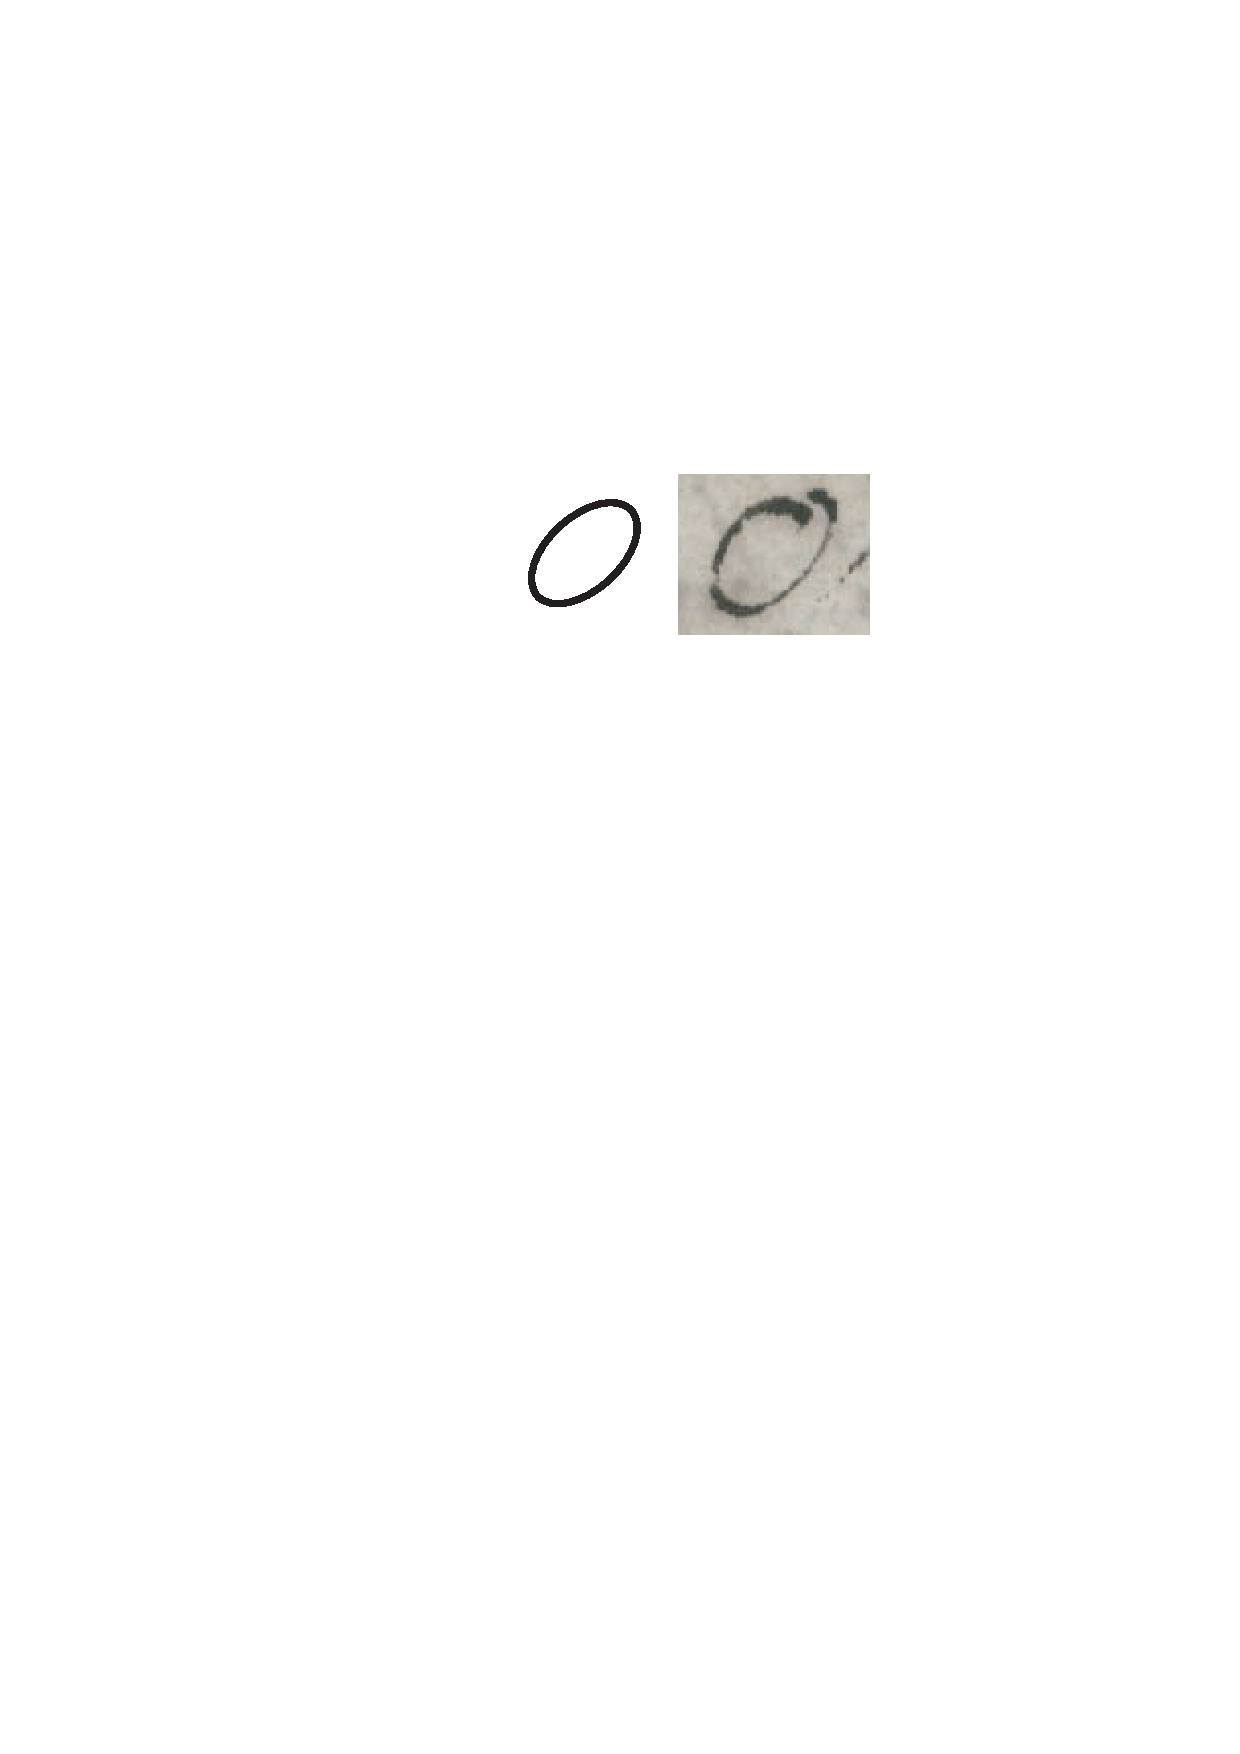
\includegraphics[width=0.15\textwidth]{images/lh0040104b_011v4.pdf}
sed in quaeaciculae caput immittendo non admodum alte penetrabat, vesica intus erat quae oesophagum a spina dorsi separabat, eratque accurate in medio corporis et anfractuosa ad omnes cavitates replendas; erant et aliae membranae omnes interiores partes involventes et simul jungentes, erat et dia$\phi$ragma quod nihil supra se continebat, praeter cor, oris cavitatem et caput. Nec dubitavi quin cursus sanguinis in ejusmodi piscibus sit, a corde per branchias ad caput atque inde per anteriorem spinae partem versus caudam itemque ad lienem, atque ex liene ad hepar et intestina ex intestinis etiam succum ciborum ad hepar, et inde simul cum sanguine ad cor. In branchiis vero etiam auditus organum esse potest, sunt enim ex parte osseae; nervi veniunt ex cerebro per posteriorem spinae partem non per ejus medium.
\pend
\pstart%
Cum vasa urinae vasis spermaticis in omnibus animalibus sint cunjuncta non videtur alia esse causa distinctionis inter marem et foeminam, quam quod haec prius urinam emiserit, quam spiritus prolifici rudimentum;
hic contra. Nec mirum, quod omnia fere animalia generent, quae enim generare non possunt, non etiam generantur nec proinde reperiuntur in mundo.
[12~r\textsuperscript{o}]
\pend%
\count\Bfootins=1500
\count\Cfootins=1500
\count\Afootins=1500